\chapter{Interazione disco-pianeta}

\begin{wrapfigure}[26]{l}{0.4\textwidth}
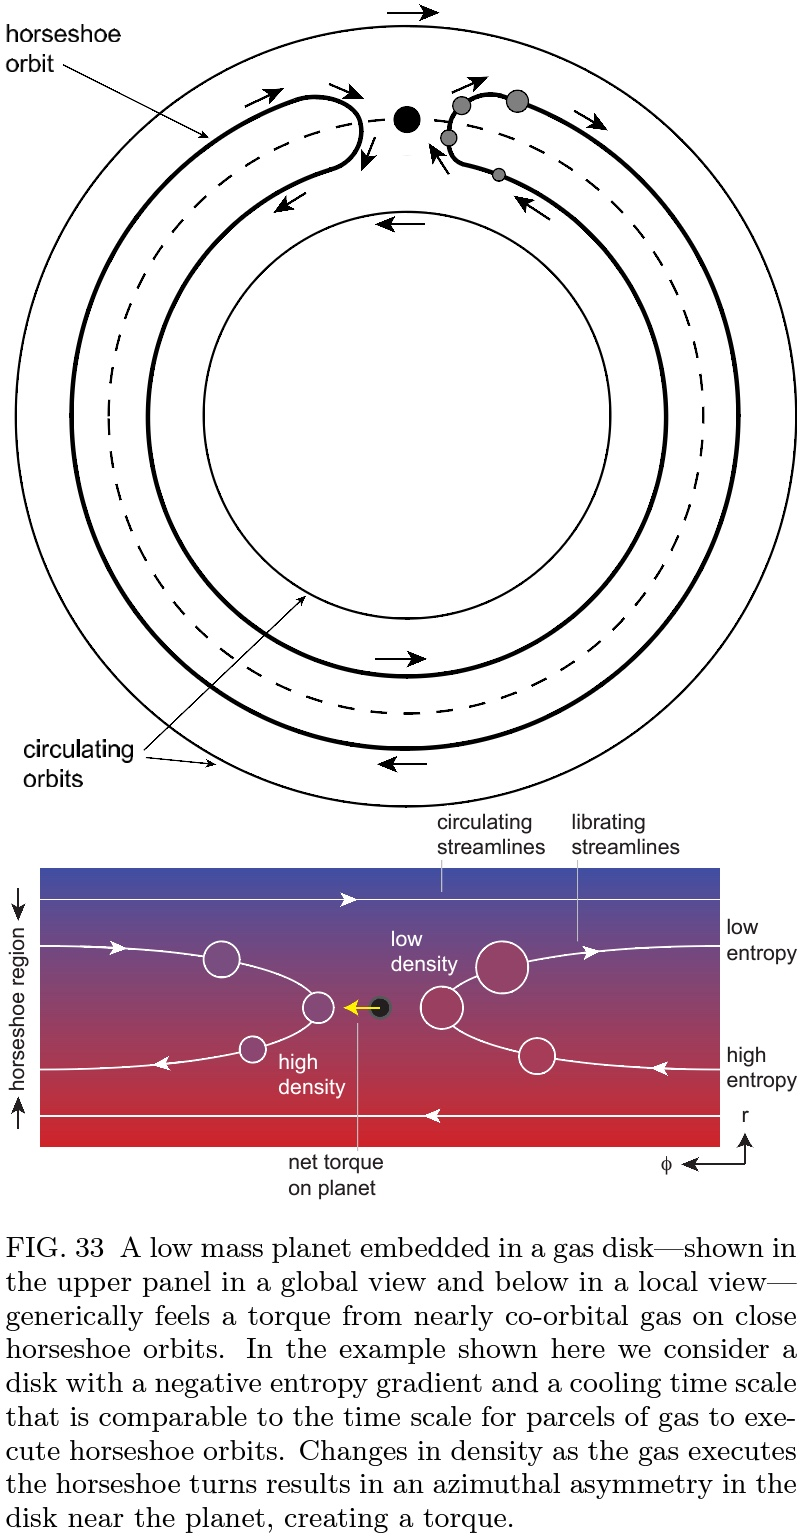
\includegraphics[trim={0cm 11cm 0 0},clip, keepaspectratio, width=0.39\textwidth]{corotation}
\caption{In alto: Orbite periodiche e librazione delle particelle di gas del disco. In basso: Asimmetrie tra gli U-turn che precedono/seguono il pianeta. Da \cite{armitage2007lecture}.}\label{fig:corotation}
\end{wrapfigure}

Considero in maniera schematica lo scambio di momento angolare tra pianeta e disco usando l'approssimazione impulsiva, dove si considera la traiettora di un elemento di fluido che interagisce col pianeta e integrando sui parametri d'impatto ammissibili, oppure descrivendo in approssimazione lineare l'interazione tra onde di densit\'a e pianeta. L'analisi lineare delle perturbazioni generate dal pianeta fornisce l'espressione analitica dei momenti torcenti esercitati dal disco sul pianeta alle risonanze di Lindblad e di corotazione.

Per pianeti massicci la risposta del disco non \'e pi\'u lineare: il momento angolare viene assorbito in prossimit\'a delle risonanze di Lindblad e si crea un gap nel disco. Il passaggio a regimenon lineare nella regione di corotazione avviene su tempi minori del tempo-scala di librazione:
\begin{equation}
\tau_{lib}\propto\frac{a_p}{\Omega_px_s}
\end{equation}
con:
\begin{equation}
x_s\propto a_p\sqrt{\frac{q}{h}}, \ h=\frac{H}{a},\ q=\frac{m_p}{M_*}
\end{equation}

I risultati riportati sono per disco isotermo:nei dischi reali si pu\'o avere migrazione stocastica e zone di concentramento dovute a transizioni di opacit\'a.

\begin{workout}[Migrazione: situazione complessa]
Armitage07 pg 57-58
\end{workout}

\begin{workout}[Migration refs]
lecture 14 (Henning Benz Klahr mordasini)
Terquem papaloizou (planet formation and migration) pg 43
Planet-disk interaction and orbital evolution
Refs: \cite{ward1997protoplanet}, \cite{terquem2000disks}, \cite{menou2004low}, (
Planet-disk interaction and orbital evolution (kley Nelson 2012), 
Baruteau 2016)
crida06: On width and shape of gaps in PPD,crida phd, 
Trilling 98:Orbital evolution and migration of giant planet: modellingextrasolar planets (Angular momentum injection rate, torque from spinning star, Impact of planet migration models on planetary populations)
Dittkrist 14: Impact of planetsmigration models n planetarypopulation (Migration II inward/outward: non equilibrium gas flow, problem of isothermal disk migration timescale: migration I regime, Fig 7;
Refs: On the tidal interaction between protoplanets and the primordial solar nebula. II - Self-consistent nonlinear interaction (1986)
Non-linear. For larger planet mass, when disk density distro is changed cons., the linear hteory is no more adeguate. If angular momentum isdeposited locally (viscous dissipation/shock waves)  the disk receeds from planets
Ida-lin04: angular momentum trasport in viscous accretion disk without planets that in type II migration act as relays that transmit angular momentum at that rateacross their gap via tidal torques.
Alibert05: the planet follow the gas except when massive than local disk.
Duffell14, Durmann kley 15: questioning that migration II follows viscous evolution of the disk but due to torque??
Planet-disk interactions: exchange of angular momentum. Low mass planet-linear theory.(''Planet-disk interactions and orbital evolution'')
Low mass planets: Lindblad and corotation torque. Rapid migration of intermediate mass planets. Gap forming massive planets: slower migration determined by viscous evolution of disk. (Role of disk self-gravity and MHD turbulence as function of planet mass).
\end{workout}

\begin{workout}[Bernoulli -Fluid dynamics (Landau)]
Bernulli: lungo linea di flusso $\frac{1}{2}v^2+w+gz=\const{}$
\end{workout}

\begin{workout}[Not isoentropic flow (pg14) -Fluid dynamics (Landau)]
$\TDof{t}(\frac{\vec{\omega}\cdot\nabla s}{\rho})=0$
\end{workout}

\begin{workout}[Flow between rotating cylinder (pg55) -Fluid dynamics (Landau)]
Navier-Stokes equation gives
\begin{align*}
&\TDy{r}{P}=\frac{\rho v^2}{r}\\
&\TtwoDy{r}{v}+\frac{1}{r}\TDy{r}{v}-\frac{v}{r^2}
\end{align*}
cercabdo soluzione della forma $r^n$ l'ultima ha soluzione: $v=ar+\frac{b}{r}$.
a,b determinate da condizioni al contorno
\end{workout}


\begin{workout}[migration and disk parametrizzation]
Toward deterministic model of planetary formation IV: effects of type-I migration (highly optically thin disk)
\end{workout}

\begin{workout}[disk torque]
Orbital evolution and migration of giant planets: disk evolution and torque;
\end{workout}

\begin{workout}[Horseshoe drag refs]
Horseshoe drag in three-dimensional globally isothermal disks (masset15)
mordasini dittkrist14 (width of horseshoe region)
On horseshoe drag of a low-mass planet. I-migration in isothermal disks: relaxation of globally isothermal HP 6 (pg 29);Inroduction and first torque expression (pg1-14); 
\end{workout}

\begin{workout}[type I: migration is too fast]
magnetic fields cloud produce stocasticity and thus s migration: nelson papaloizou 04, laughlin 04
laminar/turbulent disk: nelson 05 - tidal torque on fluctuations
global magnetic fields terquem 03
global distortion (non zero eccentricity): papaloizou 02
opaciy transitionmenou goodman 04
instabilities in inviscid gap enge: koller 03
\end{workout}

\begin{workout}[planetary migration usefull formulae]
\begin{align}
\TDy{t}{j}=1/2\sqrt{GM_*/r}\TDy{t}{r}
\end{align}
Il disco di accrescimento esercita momento torcente sul pianeta che produce un trasferimento di momento angolare dal pianeta al disco $\Lambda(a,R)$
\begin{align*}
&J=M_p\sqrt{GM_*a_p}\\
&\TDy{t}{a}=2a_p\frac{\Gamma_t}{J}=-(\frac{a}{GM_*})(\frac{4\pi}{M_P})\int_{r_{int}}^{r_{out}}r\Lambda\Sigma\,dr
\end{align*}
$r_{int}, r_{out}$ inner/outer disk radius (rif to disk ar planet)
\end{workout}


\begin{workout}[M14:type I]
below few tenth of $\mearth{}$.
Linblad torque: inside/outside corotation region.
corotation torque: depends on thermodynamics regime of interaction between planet/disk.
\end{workout}

\begin{workout}[Corotation torque: non-linear (except early stages) horseshoe drag.]
(On horseshoe drag of low-mass planets)
Jump in angular momentum of particles undergoing U turn, before/after planets (in librating orbit).
ward91, masset 01,02, masset papaloizou 03, paardekooper papaloizou 09.
Linear analysis: corotation torque arise from anulus of radial extent H around corotation, launch of evanescent waves in coorbital region; horseshoe analysis consider horseshoe region.
\end{workout}

\begin{workout}[Horseshoe drag]
Horseshoe drag low-mas planet: migration in isothermal disk (casoli Masset 09): torque, width of corotation region
\end{workout}

\begin{workout}[type I: planets not massive enough to open a gap]
Linear response of disk to orbiting planets - perturbazione del pianeta sul disco si propagano come onde di densit\'a fuori dalle risonanze e come onda evanescente fra le risonanze nella regione di corotazione. Il protopianeta esercita un momento torcente sulle onde di densit\'a cha assieme  a quello di corotazione \'e responsabiledello scambio di momento angolare tra disco mkoto orbitale del pianeta: la maggior parte del toque \'e esercitato vicino alle risonanze di L./corotazione dove la lunghezza d'onda della perturbazione \'e lunga (lontano la perturbazione ha lunghezza d'onda breve: contributo mediato a zero): terquem00.
Il momento pu\'o essere calcolato facendo una analisi lineare delle onde eccitate in 2D/3D o sommando i momenti torcenti puntiformi esercitati alle risonanze di lindblad/corotazione.
\begin{align}
&t_I\propto J/\dot{J}\propto(H/a)^2\\
&t_e\propto e/\dot{e}\propto(H/a)^4
\end{align}
\end{workout}

\begin{workout}[M14:type II and outward migration]
adiabatic and local isothermal disk: pardekooper 10/11
Type II planet-dominated for mass $100\mearth{}$.
$\dot{a}_p\propto v_g$: ??
Veras armitage 04 (exoplanets with $a>20au$): outward migration seldom important, radius velocity reversal when type II migration occure $R_{mvc}$ is outside them.
\end{workout}

\vspace{2.5cm}

\section{Migrazione tipo I: pianeti piccola massa - comportamento lineare.}

\subsection{Risonanze di Lindblad}
%chapter 6 (gemelli.spacescience)
Considero un disco kepleriano ed espando il potenziale generato da un pianeta, periodico in $\phi_p=\Omega_pt$:
\begin{align}
&\psi_p(r,\phi,t)=-\frac{Gm_p}{|\vec{r}_p(t)-\vec{r}|}=\sum_{m=0}^{\infty}\psi_m(r)\cos{m[\phi-\phi_p(t)]}
\end{align}
Attorno all'orbita del pianeta si hanno orbite risonanti per elementi di fluido del gas. La condizione di risonanza \'e
\begin{align}
&\pm\kappa_0=m(\Omega-\Omega_p)\\
&r_L=(\frac{m}{m\pm1})\expy{2/3}a
%\kappa_0^2=\frac{2\Omega}{r}\TDof{r}(r^2\Omega)
\end{align}
dove $\kappa_0=\Omega$ per disco Kepleriano \'e frequenza epiciclica e $r_L$ posizione delle risonanze.

%%RMM disco pianeta: gli elementi di fluido descrivono m orbite attorno al pianeta il pianeta compie $m\pm1$ orbite

Per tenere conto della pressione introduco l'altezza scala del disco $c_s=H\Omega$. La posizione della risonanza \'e allontanata:
\begin{equation}
m[\Omega(r_L)-\Omega_p]=\mp\Omega(r_L)\sqrt{1+m^2(H/r)^2}
\end{equation}

Inoltre le risonanze rimangono a distanza finita dal pianeta:
\begin{align}
%&m(\Omega(r)-\Omega_p)=\sqrt{\kappa^2(r)(1+\xi^2)}\\
&\lim_{m\to\infty}r_L=r_p+\frac{2H}{3}
\end{align}
%dove $\xi=\frac{mc_s}{\Omega r}$, $c_s=H\Omega$.

\subsection{Momento torcente dovuto alle risonanze di Lindblad}
Il momento torcente esercitato dal disco sul pianeta \'e
\begin{equation}
\Gamma_L^{int/est}=-\int_{int/est}\Sigma(\vecp{r}{F})\,df=\int_{int/est}\Sigma(\vec{r}\wedge\nabla\psi_p)\,df=\int_{int/est}\Sigma\PDy{\phi}{\psi_p}\,df\label{eq:pd-torque}
\end{equation}
$\Sigma$ densit\'a superficiale,  $\vec{F}$ forza per unit\'a di massa, $df$ elemento di superficie.
%Linear. Occur if $R_H$ is smaller then H, disk scale heigth, and if viscous torque are dominant compared to gravitational torque.
(Integrando l'equazione \eqref{eq:pd-torque} si ottiene) L'espressione del momento torcente esterno/interno
\begin{equation}
%\Gamma_m^L=\left.\sign{(\Omega-\Omega_p)}\frac{\pi^2\Sigma}{3\Omega\Omega_p}(r\TDy{r}{\psi_m}+\frac{2m^2(\Omega-\Omega_p)}{\Omega}\psi_m)^2\right|_{r=r_L}
\Gamma_L^{int/est}\propto q^2\Sigma r^4\Omega^2(\frac{r}{H})^3
\end{equation}\label{eq:torqueimp}
con $q=M_p/M_*$, infine una stima del momento torcente differenziale delle risonanze di Lindblad \'e fornito da \cite{tanaka2002three}:
\begin{equation}
\Gamma_L^d\propto q^2\Sigma r_p^4\Omega_p^2(\frac{H}{r})\expy{-2}
\end{equation}
per disco isotermo infinitamente sottile.

\subsection{Momento torcente dovuto alle risonanze di Corotazione}

La regione di corotazione \'e definita da $\Omega(r)-\Omega_p=0$ cio\'e il potenziale del pianeta ruota alla stessa frequenza del fluido.

Il momento torcente dovuto alle risonanze di corotazione \'e
\begin{equation}\label{eq:corotorquelinear}
\Gamma_C^m\propto m[\frac{\psi_m}{\TDy{r}{\Omega}}\TDof{r}(\frac{\Sigma}{B})]_{r_c}
\end{equation}
dove $\psi_m$ \'e la m-esima componente del potenziale e $2B$ la vorticit\'a del flusso; la regione di corotazione \'e divisa in m isole di librazione.
Il gradiente di $\Sigma/B$ va rapidamente a zero se non mantenuto da adeguata viscosit\'a.
%$\nabla\wedge\vec{r}=vorticit\'a$

\subsection{Velocit\'a migrazione tipo I}

Utilizzando la stima di \cite{tanaka2002three} si trova il tempo caratteristico per migrazione tipo I

\begin{equation}
\tau_I=\frac{r_p}{|\dot{r}_p|}=\frac{\dot{J}_p}{\Gamma_{dL}}=\frac{1}{2.1+1.1\gamma}\frac{M_*}{M_p}\frac{M_*}{r_p^2\Sigma(r_p)}(\frac{c_s}{r_p\Omega_p})^2\frac{1}{\Omega_p}
\end{equation}
da cui risulta pr disco protoplanetario con $\Sigma(r)=1500(r/\SI{5}{\astronomicalunit})\expy{-3/2}\si{\kilo\gram\per\square\meter}$ a $T=\SI{130}{\kelvin}$ per pianeta di massa terrestre a \SI{5}{\astronomicalunit} un tempo di migrazione $\tau_I\approx\SI{8e5}{\year}$: molto minore del tempo di vita del disco.

Il momento torcente
\begin{workout}[M14:type II and outward migration]
Freuenza epiciclica
\begin{equation}
\kappa^2=4\Omega^2+r\TDy{r}{\Omega^2}
\end{equation}
\end{workout}


\begin{workout}[Migration I in isothermal disk: pressure.]
Low mass planet in isothermal disk: linear analysis of perturbed flow.
When pressure can't be neglected the resonance condition becomes $m(\Omega(r)-\Omega_p=\sqrt{\kappa^2(r)(1+\xi^2)}$ where $\xi=\frac{mc_s}{\Omega r}$ where we used isothermal sound speed and let $c_s=H\Omega$: for $m\to\infty$ L. res position becomes $r_L=r_p+\frac{2H}{3}$ (torque cutoff).

Linear. Occur if $R_H$ is smaller then H, disk scale heigth, and if viscous torque are dominant compared to gravitational torque.
Subtypes: locally isothermal, adiabatic, un/satured-corotation torque: cooling behaviour of gas (Baruteau masset08, Casoli masset 08, paardekooper10,kley 09); timescales: dittkrist 14.
Migration timescale in isothermal approx (ida lin 08 a:):
\begin{align*}
&\tau_I=\frac{1}{2.728+1.082p_{\Sigma}}(\frac{c_s}{a_p\Omega})^2\frac{M_*}{M_p}\frac{M_*}{a_p^2\Sigma_g}\Omega\expy{-1}\\
s&\dot{a}_p=-\frac{a_p}{\tau_I}
\end{align*}
Paardekooper10, Dittkrist14: total torque $\Gamma_t=\frac{1}{\gamma}(C_0+C_1p_{\Sigma}+C_2p_T)\Gamma_0$ where $C_i$ depends upon sub-regime.
Benitez Llambay 15: heating torque, Paardekooper14 Pierens 15: dynamic corotation torque.
\end{workout}

\section{Migrazione tipo II:pianeti massicci.}

Per pianeti massicci il trasporto viscoso di momento angolare non \'e abbastanza efficiente quindi si forma un gap attorno al pianeta: questo \'e detta migrazione di tipo II. il pianeta prende momento dal disco esterno (dovuto al flusso viscoso) e cede quello richiesto al disco esterno dal trasporto viscoso: normalmente il bilancio \'e negativo quindi il pianeta migra verso l'interno.

\subsection{Approssimazione impulsiva}

%Lin papaloizou 79
\begin{wrapfigure}[10]{l}{0.45\textwidth}
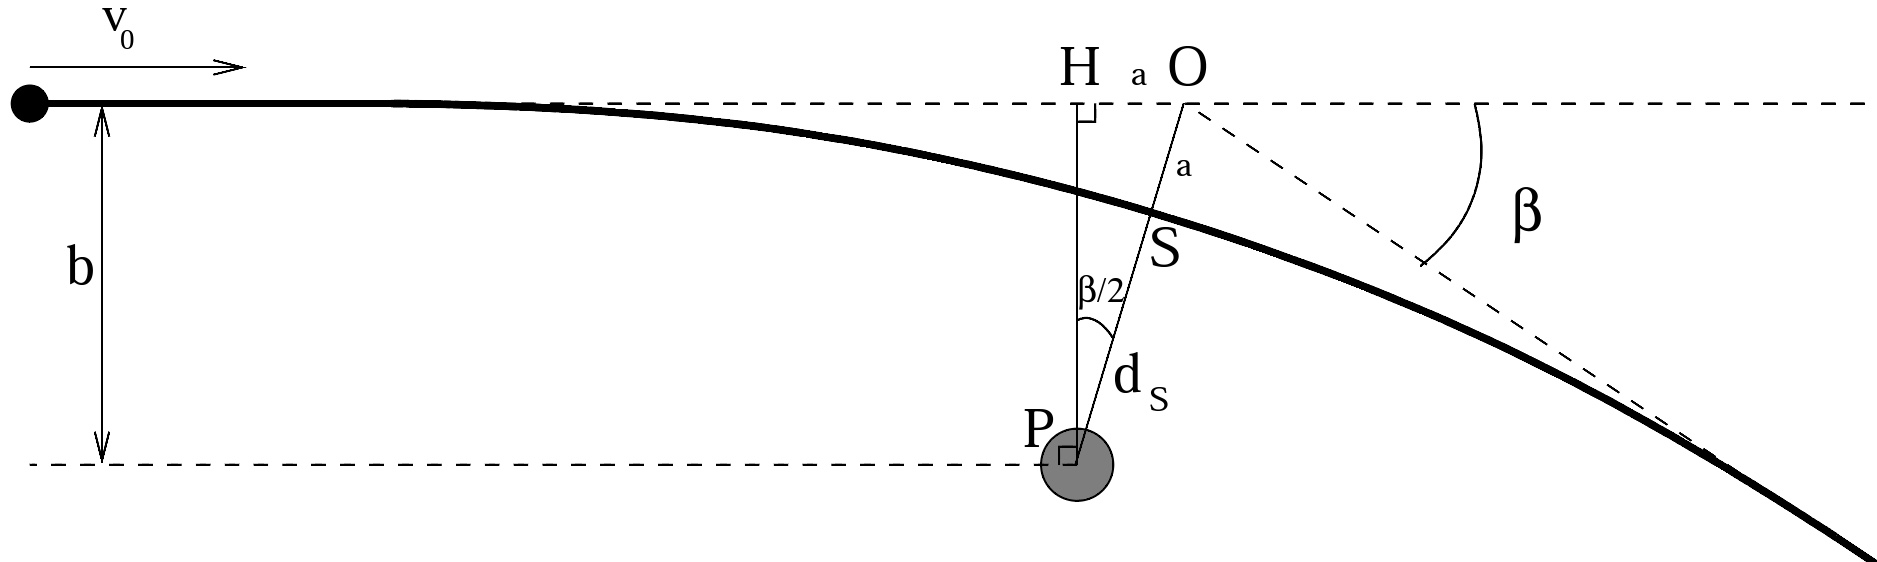
\includegraphics[width=0.45\textwidth]{impulseapprox}
\caption{Schema approssimazione impulsiva.}\label{fig:impulseapprox}
\end{wrapfigure}

L'approssimazione impulsiva \'e valida per incontri veloci dove la velocit\'a relativa tra elemento di fluido e pianeta \'e maggiore della velocit\'a del suono $c_s$:
\begin{equation}b_{min}=c_s|\TDy{r}{\Omega}|\expy{-1}=\frac{2}{3}H\end{equation}

In questa approssimazione posso trascurare il moto del pianeta attorno alla stella. La traiettoria di un elemento di fluido \'e deviata di un angolo
\begin{equation}
\beta=\arctan{\delta v/v_0}=\arctan{(\frac{GM_p}{bv_0^2})}
\end{equation}
$v_0=r(\Omega-\Omega_p)$ velocit\'a relativa fluido-pianeta, b parametro d'impatto.

Trasferimento di momento angolareper unit\'a di massa rispetto alla stella:
\begin{align}
&\delta j=rv(\cos{\beta}-1)=-2r\frac{G^2M_p^2}{b^2v^3}
\end{align}
Il disco cede momento angolare al pianeta con rate
\begin{equation}
\frac{\delta j}{\delta t}=\frac{\delta j}{2\pi/|\Omega-\Omega_p|}
\end{equation}

Infine il momento torcente totale esercitato dal pianeta sulla porzione esterna di disco che si estende da $r_p+\Delta$ a infinito \'e
\begin{equation}
\Gamma_{imp}=\int_{r_p+\Delta}^{\infty}\int_0^{2\pi}\frac{\delta j}{\delta t}\Sigma r\,d\theta\,dr\propto\Sigma q^2r_p^4\Omega_p^2\frac{r_p^3}{\Delta^3}\label{eq:torqueimp}
\end{equation}

Per materia in orbita circolare interna/esterna al pianeta il trasferimento \'e positivo/negativo.
%per disco esterno all'orbita l'espressione \'e la stessa con segno invertito perch\'e il disco or a \'e pi\'u lento del protopianeta.

\subsection{Regime non lineare: fromazione di gap attorno al pianeta}
%Formazione di gap per dischi tipici sopra massa di saturno.
%Viscous torque in keplerian disk: $T_{\nu}=3\pi r_0^2\Omega_0\Sigma\vu$.

Il limite del regime lineare  \'e raggiunto quando il momento torcente dovuto al potenziale del pianeta \'e pari a quello dovuto alla viscosit\'a del disco:
\begin{equation}
\Gamma_g(\Delta)+\Gamma_{\nu}(r_p+\Delta)=0
\end{equation}
con $\Gamma_g$ dato da o \eqref{eq:torqueimp} dove si era usata la distanza minima $\Delta=\frac{2}{3}H$.

Le condizioni necessarie per apertura gap sono (\cite{papaloizoulin1984})
\begin{align}
&R_H>H\\
&\frac{\nu}{r_p^2\Omega_p}<0.0887q^2(\frac{r_p}{H})^3
\end{align}
la prima impone che influenza gravitazionale del pianeta sia maggiore dell'altezza caratteristica del disco, la seconda che $\Gamma_g>\Gamma_{\nu}$.

\subsection{Tempi caratteristici migrazione tipo II}

Quando la massa del pianeta non eccede la massa locale del disco il tempo scale di migrazione \'e
\begin{equation}
t_{II}(yr)=\frac{1}{3\alpha}(\frac{a}{H})^2\Omega\expy{-1}=0.05/\alpha(a/H)^2(a/au)\expy{3/2}
\end{equation}
per $H/a\approx0.1$, $\alpha=\numrange{e-3}{e-2}$ a $a=1-5 au$ si ha $t_{}=10^3-10^4yr$.

\begin{workout}[approx impulsiva e regime non lineare]
(The interaction is frictional with interior speeding up protoplanet while exterior slowing down; viscous interaction with disk return mass element in circular orbit)
Il calcolo esatto che tiene conto del fatto che siamo in SR rotante (LP93) introduce fattore correttivo $K_0=4/9[2K_0(2/3)*K_1(2/3)]^2$.
La velocit\'a relativa \'e $u=a|\Omega_p-\Omega_g$ e dato che l'interazione avviene vicino al pianeta $|\Omega_p-\Omega_g|\approx3/2b\Omega_p/a$.
Rate trasferimento momento angolare tra interno del disco e pianeta
\begin{equation}
\TDy{t}{J}=\int_{b_{min}}^{+\infty}a\Sigma\Delta J|\Omega_p-\Omega_g|\,db
\end{equation}
Il parametro d'impatto minimo \'e l'assunzione implicita di un gap nel disco a assenza di materia nella regione di corotazione (discussione applicabilein regime non-lineare)
Formazione gap: perch\'e il gap si stazionario il momento scambiato nell'interazione disco-pianeta deve essere almeno quello trasportato dal moto viscoso del disco:
\begin{equation}
\TDy{t}{J}|_{visc}=3\pi\nu\Sigma a^2\omega
\end{equation}
deve essere quindi $\TDy{t}{J}|_{visc}<\TDy{t}{J}$
Cut-off: $b_{min}\approx H$, la pressione smorza effetti su scala pi\'u piccola; regime non-lneare, richiesto per gap formation, lunghezza-scala del flusso non minore di $r_H$: predndendo $b_m=2r_h$ si ha
\begin{equation}
\frac{M_p}{M_*}>\frac{40\nu}{a^2\omega}
\end{equation}
\end{workout}


\section{Migrazione tipo III}

Esistono condizioni per cui il momento torcente generato nella zona di corotazione diventa dominante.

\subsection{Momento torcente generato nella regione di corotazione}

L'espressione \ref{eq:corotorquelinear} \'e valida per $t\ll\tau_{lib}$, dal momento che si instaurano orbite di librazione nel disco l'espressione del momento torcente diventa
\begin{equation}
\Gamma_C\propto x_s^4\Omega_p^2\Sigma\TDly{r}{(\frac{\Sigma}{B})}\label{eq:horsetorque}
\end{equation}

\begin{workout}[horseshoe drag: streamline, nonlinear. corotation torque: linear]
paardekooper papaloizou 09: '' On corotation torque, horseshoe drag and the possibility of sustrained stalled or outward protoplanetary migration''.
masset 06: ''On the migration of protogiant solid cores''
\end{workout}

Il momento torcente dovuto al flusso di materia causato dalla migrazione \'e
\begin{equation}
\Gamma_{III}=2\pi\Sigma_s\dot{a}_p\Omega_pa_p^3x_s
\end{equation}

\begin{workout}[corotation torque from ''disk planet interction'']
The torque excerted by all fluid elements is (Goldreich tremaine79, Ward 91,92)
\begin{equation}
T_C3/4x_s^4\Omega_p^2\Sigma\TDly{r}{\Sigma/B}
\end{equation}
old from ''disk-planet interactions''
\begin{equation}
\Gamma_m^C=\left.\frac{m\pi^2}{2}\frac{\psi_m}{r\TDy{r}{\Omega}}\TDof{r}(\frac{\Sigma}{B})\right|_{r=r_C}
\end{equation}
$B=\frac{\kappa^2}{4\Omega}$ \'e la seconda costante di Oort (rappresenta componente z della vorticit\'a $\nabla\wedge\vec{v}|_z$).
infine il momento torcente totale \'e
\begin{equation}T_I=\sum_{m}^{int}\Gamma_m^L+\sum_{m}^{out}\Gamma_m^L+\sum_{m}\Gamma_m^C\end{equation}

Corotation torque saturation depends upon $\tau_{nlib}/\tau_{vis}$: over timescale long rel. to librration time angular momentum exchanged between planet-disk average to zero.
\end{workout}

\subsection{Corotation torque in accretion disk and migration 3 type}
%Viscosity desaturate,crida pg 39: 
Sia $b_0=r-r_p$ la distanza dal pianeta di un elemento di fluido in congiunzione
$\tau\approx2\pi/|x_s\TDy{r}{\Omega}|=4\pi r_p/(3x_s\Omega_p)$


\begin{workout}[type III and coorbital torque]
COnsidero un pianeta migrante: quando il gap \'e parziale materiale percorre l'orbita ed esercita momento t, positive/negative feedback.
Per un pianeta che migRA VERSO L'ESTERNO SI HA
$2\pi\Sigma R\TDy{t}{R}$ \'e il flusso di massa che impartisce momento per unit\'a di massa al protopianeta quando la materia attraversa la regione di corotazione di spessore w, $w\omega/2$: con $w=2H$ si ha
\begin{align}
F_{cr}=2\pi R\Sigma\omega^2 H^2\frac{1}{c_s}\TDy{t}{R}=1/2M_d\omega\TDy{t}{R}\\
F_{crb}=-1/2M_b\omega\TDy{t}{R}
\end{align}
dove la seconda \'e inerzia (??) massa legata al pianeta.
quazione del moto:
\begin{equation}
1/2M_pa\omega\TDy{t}{a}=1/2(M_d-M_b)a\omega\TDy{t}{a}+T_{ext}
\end{equation}
\end{workout}

Per pianeti di massa intermedia si pu\'o instaurare un regime di migrazione veloce detta mifìgrazione di tipo III dove il momento torcente esercitato sul pianeta \'e
\begin{equation}
%\Gamma_{flow}=2\pi\Sigma_s\dot{a}_p\Omega_pa_p^3x_s
\Gamma_{flow}\propto\dot{a}_p\Omega_pa_p\delta m
\end{equation}
dove $\delta m$ esprime la perturbazione della massa presente nella regione di corotazione dovuta al pianeta.
%\section{Evoluzione elementi orbitali durante migrazione}

\begin{workout}[Eccentricity and inclination evolution]
Refs:armitage 17 ''lecturea''
Planet-disk interactions: normal, tangential, radial forces. eccentricity and inclination evolution. (‘’Planet-disk interactions and orbital evolution’’)
Decomposition of planet’s potential: non-circular orbit
\begin{align*}
&\psi_p(r,\phi,t)=-\frac{Gm_p}{|\vec{r}_p(t)-\vec{r}|}=\sum_{m=0}^{\infty}\sum_{n=-m}^m\psi_{m,n}(r)\cos{m\phi+(n-m)\Omega_pt]}
\end{align*}
Eccentricity damping.
For each m,n there are 3 resonant locations: external L resonance act to increase, corotation res. to damp (if unsaturted), and coorbital L res damp $e_p$. Linear analysis for low mass planets indicates rapid exponential damping of $e_p$:
\begin{align*}
&\TDy{t}{e_p}\propto-e_p,\ \tau_e\approx(\frac{H}{r})^2\tau_{mig}\\
&e_P>\frac{H}{r}: \TDy{t}{e_p}\propto-e_p\expy{-2}
\end{align*}
Risultati analoghi per inclinazione.	
\end{workout}


%\section{Altre interazioni che producono migrazione}


\begin{workout}[mass loss and conservation of angular momentum]
Orbital evolution and migration of giant planets: mass loss and conservation of angular momentum.
\end{workout}

\begin{workout}[torque from spinning star]
Orbital evolution and migration of giant planets: torque from spinning star
\end{workout}

\begin{workout}[planet overlflowing roche lobe migrate outward]
trilling 98:n During mass flow planet moves outward to conserve angular momentum
\end{workout}

\begin{workout}[Other (than?) types of migration]
planet-planet scattering (rasio ford 96, kozai (nagasawa 08, tidal interactions with gas disk (goldreich tremaine 80, tanaka 02))
\end{workout}

\begin{workout}[planet locked in resonances]
as solar system satellites: goldreich 65.
N-body, resonanceand migration: The dynamics of two massive planets on inclined orbits (Veras Armitage 04)
orbital migration occurring at different rates due to disk parameters can produces convergent migration and locking into mean motion resonances.
kley 04
aligned absidal line: papaloizou 03
\end{workout}
